\documentclass[tikz, border=5mm]{standalone}
\usetikzlibrary{calc, shapes.geometric}

% Macro para insertar secuencialmente los nodos (Sin el círculo de búsqueda).
% Argumentos:
% #1: Número de paso en el que se activa
% #2: Nombre del nodo (ej. q1)
% #3, #4: Coordenadas X e Y
% #5, #6, #7: Nombres de los 3 vecinos más cercanos a conectar
% #8: Etiqueta textual (ej. $q_1$)
\newcommand{\drawAddition}[8]{
    \ifnum\step<#1\relax
        % Si el paso actual es menor al paso de activación, no se dibuja nada
    \else
        \coordinate (#2) at (#3, #4);
        \ifnum\step=#1\relax
            % Si es el paso EXACTO de activación: Dibujar como "NUEVO" (Rojo)
            % 1. Dibujar aristas nuevas
            \draw[new edge] (#2) -- (#5);
            \draw[new edge] (#2) -- (#6);
            \draw[new edge] (#2) -- (#7);
            % 2. Dibujar el nodo
            \node[new node] at (#2) {};
            \node[above right, font=\tiny\bfseries, red!80!black] at (#2) {#8};
        \else
            % Si es un paso posterior: Integrar al grafo "BASE" (Gris/Azul)
            \draw[base edge] (#2) -- (#5);
            \draw[base edge] (#2) -- (#6);
            \draw[base edge] (#2) -- (#7);
            \node[base node] at (#2) {};
        \fi
    \fi
}

\begin{document}
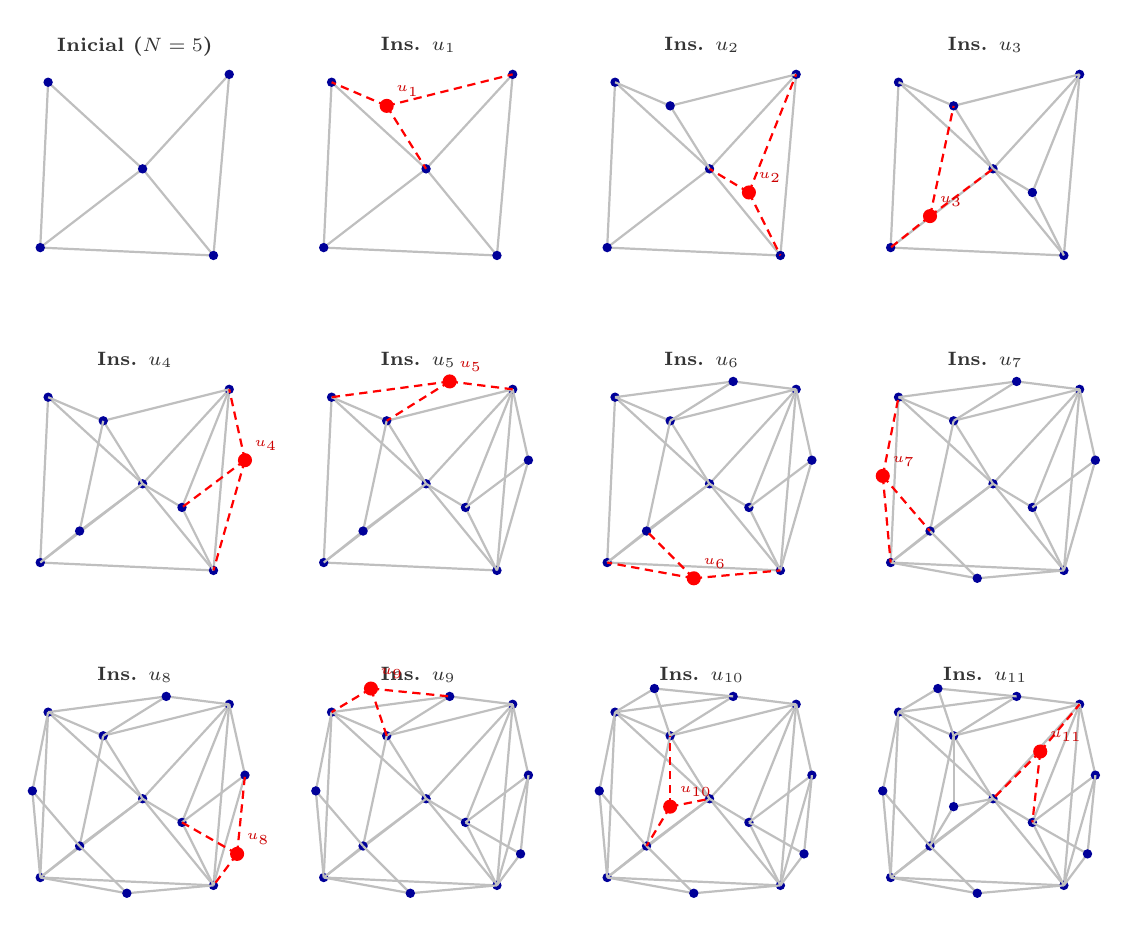
\begin{tikzpicture}[
    base node/.style={circle, fill=blue!60!black, inner sep=1.2pt},
    new node/.style={circle, fill=red, inner sep=1.8pt},
    base edge/.style={thick, black!25},
    new edge/.style={thick, red, densely dashed}
]

% Bucle para generar la cuadrícula de 12 paneles (3 filas x 4 columnas)
\foreach \step/\xshift/\yshift/\title in {
    1/0/8.0/{Inicial ($N=5$)},
    2/3.6/8.0/{Ins. $u_1$},
    3/7.2/8.0/{Ins. $u_2$},
    4/10.8/8.0/{Ins. $u_3$},
    5/0/4.0/{Ins. $u_4$},
    6/3.6/4.0/{Ins. $u_5$},
    7/7.2/4.0/{Ins. $u_6$},
    8/10.8/4.0/{Ins. $u_7$},
    9/0/0/{Ins. $u_8$},
    10/3.6/0/{Ins. $u_9$},
    11/7.2/0/{Ins. $u_{10}$},
    12/10.8/0/{Ins. $u_{11}$}
}{
    \begin{scope}[shift={(\xshift, \yshift)}]
        
        % 1. Caja y Título del Sub-cuadro
        %\draw[draw=black!20, fill=gray!5, rounded corners] (-0.2, -0.2) rectangle (3.4, 3.4);
        \node[font=\scriptsize\bfseries, color=black!80, anchor=north] at (1.6, 3.3) {\title};

        % 2. Coordenadas de los 5 Puntos Iniciales
        \coordinate (p1) at (0.5, 2.6); 
        \coordinate (p2) at (2.8, 2.7);
        \coordinate (p3) at (1.7, 1.5); 
        \coordinate (p4) at (0.4, 0.5);
        \coordinate (p5) at (2.6, 0.4); 

        % 3. Aristas del Grafo Base (k-NN aproximado inicial)
        \draw[base edge] (p1)--(p3); \draw[base edge] (p1)--(p4);
        \draw[base edge] (p2)--(p3); \draw[base edge] (p2)--(p5);
        \draw[base edge] (p3)--(p4); \draw[base edge] (p3)--(p5);
        \draw[base edge] (p4)--(p5);

        % Dibujar los nodos base
        \foreach \i in {1,...,5} { \node[base node] at (p\i) {}; }

        % 4. Inserciones Secuenciales (Nuevos puntos aleatorios conectados a vecinos existentes)
        % Argumentos: {Paso}{ID}{X}{Y}{Vecino1}{Vecino2}{Vecino3}{Etiqueta}
        
        \drawAddition{2}{q1}{1.2}{2.3}{p1}{p3}{p2}{$u_1$}
        \drawAddition{3}{q2}{2.2}{1.2}{p3}{p5}{p2}{$u_2$}
        \drawAddition{4}{q3}{0.9}{0.9}{p4}{p3}{q1}{$u_3$}
        \drawAddition{5}{q4}{3.0}{1.8}{p2}{p5}{q2}{$u_4$}
        \drawAddition{6}{q5}{2.0}{2.8}{p2}{q1}{p1}{$u_5$}
        \drawAddition{7}{q6}{1.5}{0.3}{p4}{p5}{q3}{$u_6$}
        \drawAddition{8}{q7}{0.3}{1.6}{p1}{p4}{q3}{$u_7$}
        \drawAddition{9}{q8}{2.9}{0.8}{p5}{q2}{q4}{$u_8$}
        \drawAddition{10}{q9}{1.0}{2.9}{p1}{q1}{q5}{$u_9$}
        \drawAddition{11}{q10}{1.2}{1.4}{p3}{q3}{q1}{$u_{10}$}
        \drawAddition{12}{q11}{2.3}{2.1}{p2}{p3}{q2}{$u_{11}$}

    \end{scope}
}

\end{tikzpicture}
\end{document}
